
 \documentclass[11pt]{article}
\usepackage{geometry}                
\geometry{letterpaper}                   

\usepackage{graphicx}
\usepackage{amssymb}
\usepackage{epstopdf}
\usepackage{natbib}
\usepackage{amssymb, amsmath}
\DeclareGraphicsRule{.tif}{png}{.png}{`convert #1 `dirname #1`/`basename #1 .tif`.png}

%\title{Title}
\author{Amr Ahmed, Elise Ledieu, Emmanuel Munich, Fran\c{c}ois Wirz}
%\date{date} 

\begin{document}


\thispagestyle{empty}

\begin{center}

\includegraphics[width=5cm]{ETHlogo.eps}

\bigskip


\bigskip


\bigskip


\LARGE{ 	Lecture with Computer Exercises:\\ }
\LARGE{ Modelling and Simulating Social Systems with MATLAB\\}

\bigskip

\bigskip

\small{Project Report}\\

\bigskip

\bigskip

\bigskip

\bigskip


\begin{tabular}{|c|}
\hline
\\
\textbf{\LARGE{The social contagion of obesity}}\\

\\
\hline
\end{tabular}
\bigskip

\bigskip

\bigskip
\bigskip
\bigskip

\LARGE{Amr Ahmed, Elise Ledieu, Emmanuel Munich \& Fran\c{c}ois Wirz}



\bigskip

\bigskip

\bigskip

\bigskip

\bigskip

\bigskip

\bigskip

\bigskip

Zurich\\
May 2014\\

\end{center}

\newpage

%%%%%%%%%%%%%%%%%%%%%%%%%%%%%%%%%%%%%%%%%%%%%%%%%

\newpage
\section*{Agreement for free-download}
\bigskip


\bigskip


\large We hereby agree to make our source code for this project freely available for download from the web pages of the SOMS chair. Furthermore, we assure that all source code is written by ourselves and is not violating any copyright restrictions.

\begin{center}

\bigskip


\bigskip


\paragraph{Amr Ahmed, Elise Ledieu, Emmanuel Munich, Fran\c{c}ois Wirz}

\end{center}
\newpage

%%%%%%%%%%%%%%%%%%%%%%%%%%%%%%%%%%%%%%%



% IMPORTANT
% you MUST include the ETH declaration of originality here; it is available for download on the course website or at http://www.ethz.ch/faculty/exams/plagiarism/index_EN; it can be printed as pdf and should be filled out in handwriting


%%%%%%%%%% Table of content %%%%%%%%%%%%%%%%%

\tableofcontents

\newpage

%%%%%%%%%%%%%%%%%%%%%%%%%%%%%%%%%%%%%%%



\section{Abstract}
\paragraph{}
Obesity is a major health concern in the US causing annual death of more than 300'000 deaths per year. World Health Organization has implemented intervention program to fight obesity.  Understanding how people become obese is key to design adequate intervention program. In 2007, Christakis and Fowler claimed that obesity spread through social networks and argued that contacts with obese person increase the likelihood of becoming obese. This claim has been subject to much controversy and was refuted by Shalizi and Thomas who highlighted the confusion made between social contagion, homophily and confounding.  Hill et al. have proposed a derived version of the SIS model, the SISa model, to allow for both social transmission of obesity and automatic infection. Using a network of 85 subjects living next to MIT for which longitudinal weight data were available, we try to fit a SISa model. However, we do not find any evidence of social contagion for obesity using conventional significance level keeping in mind the relatively limited size of our sample.

\section{Individual contributions}
\paragraph{}
We initially familiarized ourselves with the current literature and the SIS/SISa model. We agreed on the implementation and divided it into tasks. Emmanuel Munich wrote the code to read the data and perform the necessary preprocessing to it. Amr Ahmed extracted useful information from the data (like adjacency matrices). Elise Ledieu coded the regression model, while Francois plotted the Gephi plots and was responsible for integrating different pieces of code produced by different group members together. Finally, we all participated in plotting the results, discussing them and drawing conclusions from them.

\section{Introduction and Motivations}

\subsection{Introduction}
\paragraph{}
Obesity is a major health concern in the world and particularly in the US. In the US, it is estimated that obesity causes annual mortality of more than 300'000 deaths per year (Flegal, Williamson, Pamuk, & Rosenberg, 2004) despite the difficulty to precisely evaluate death directly linked to obesity. The World Health Organization defines obesity as a Body Mass Index higher than 30. WHO implemented in 2004 the WHO Global Strategy on Diet, Physical Activity and Health in order to cope with obesity. While WHO recognizes the importance of "supportive environments and communities" to fight obesity, most proposed solutions put the emphasis on an individual approach such as limiting the quantity of fat absorbed, increasing the consumption of fruits and vegetables or practising physical activity. 

\paragraph{}
Smith and Christakis  highlight the importance of the social environment associated with the physical environment as a factor of good health hinting at public health interventions which should be elaborated in harmony with the social network. Christakis and Fowler (Christakis & Fowler, 2007) argue that obesity spread  through social networks as they find that contacts with obese persons increase the likelihood to become obese. This controversial result has been debated by many including Shalizi and Thomas (Shalizi & Thomas, 2011) who point out the confusion made between homophily where subjects gather with those who resemble them, social contagion and confounding.

\paragraph{}
Hill et al. (Hill, Rand, Nowak, & Christakis, 2010) among others have extended the approach of Christakis and Fowler to allow for a transmission of obesity through social networks but also capture spontaneous non social contagion. They introduce a new model, the SISa model, derived from the classic SIS disease model to evaluate the relative effect of social and non social contagion. Hill et al. extend economic diffusion models which also include automatic diffusion by adding the possibility of recovery whereas economic diffusion are considered to be permanently acquired.

\subsection{Motivation}
\paragraph{}
It is essential to understand how people become obese to design adequate health interventions and to decide if obesity has to be tackled as a clinical issue on an individual basis or through social network to spread positive behaviour to fight obesity.

\paragraph{}
Therefore, we want to examine if social infection really plays a role in obesity spread and compare the  relative effect of social and automatic infection in obesity. We want to test if we find similar results as Hill et al. applying the SISa model to a different sample.

\paragraph{}
To answer our question, we apply the SISa model to a dataset collected by Aharony et al. (Aharony, Pan, Ip, Khayal, & Pentland, 2011) which contains one of the largest mobile data experiments done in academia to test the validity of the SISa model and estimate the model parameters in order to evaluate the social and non social aspects of obesity contagion. Aharony et al. have deployed a sensing system over 15 months to follow 130 adult members and collected their physical activity, their weight and their friendship status. We have restricted our study to a subset of 85 adults for which complete corpulence data were available.


\section{Description of the Model}

\subsection{SIS model}
\paragraph{}
We use an extension of the classic SIS model proposed by Hill et al. The SIS model is an adaptation of the SIR model developed by Kermack and McKendrick (Kermack & McKendrick, 1932). In the SIR model the population is divided into three groups: susceptible, infected, recovered. The disease is transmitted when a susceptible person enters in contact with an infected person with a so called transmission rate β. Once infected, a person can recover with a recovery rate g and then becomes completely immune to the disease. The SIS model allows to model a disease or a behaviour that can occur repeatedly meaning that recovering from the disease do not confer immunity.

\paragraph{}

In the standard SIS model, infection can only be transmitted through the contact with an infected person. The SIS model is presented in :
\begin{align}
      dI/dt  & =  \beta SI-gI \nonumber\\
      dS/dt   & =  -\beta SI+gI \\ 
      I+S & =  N \nonumber
\end{align}
where  is the number of  infected individuals, and  is the number of susceptible individuals,  is the transmission rate,  is the recovery rate and  is the total population. 

\subsection{SISa model}
\paragraph{}
Hill et al. propose an extension of the SIS model, called SISa, to allow for automatic infection without having social contact. They introduce the rate of automatic infection rate  to obtain the model described in :
\begin{align}
      dI/dt  & =  \beta SI-gI+aS \nonumber\\
      dS/dt   & =  -\beta SI+gI-aS \\
      I+S & =  N \nonumber
\end{align}

\paragraph{}
The automatic infection rate  and the transmission rate can be deduced from the transition probabilities from susceptible to infected after a time  such that:
\begin{equation}
P(S\to I,\delta t) & \sim & (a+\beta n)\delta t
\end{equation}
while the recovery rate can be deduced from the probability of transition from infected to susceptible after a time :
\begin{equation}
P(I\to S,\delta t) & \sim & g\delta t
\end{equation}

\paragraph{}

In addition, we follow Hill et al. approach and examine how a contact with an infected persons influence the transition between states.

\section{Implementation}

\subsection{Data description}
\paragraph{}
In order to implement the SISa we searched for a longitudinal dataset with similar properties as the Framingham Heart Study dataset used by Hill et al. We used the Friends and Family dataset collected by Aharony et al. The dataset consists of 130 subjects who all belong to a young residential community with at least one family member affiliated to MIT. The data were collected from October 2010 to May 2011 and an intervention program was carried out from October to December 2010. We have therefore decided to restrict our study to a subsample of the data in which there was no intervention program in place and have therefore excluded the period running from October 2010 to December 2010. 

\paragraph{}

One difficulty encountered was to harmonize the different files of the Friends and Family dataset which had to be cross-checked.

\subsubsection{Measure timing}
\paragraph{}
We have encountered an issue regarding the timing of the examinations as subjects have not been surveyed at the same exact day as the friendship was measured. We have therefore interpolated the data to solve this problem.

\subsubsection{Network description and analysis}
\paragraph{}
Subjects reported their self-perceived closeness to other egos on a scale from 0 to 7 where a number strictly higher than 2 stands for close friendship enabling us to build a binary adjacency matrix over time where a 1 stands for close friendship.

\paragraph{}

Furthermore, we have analyzed additional properties of the network, namely its degree distribution, its diameter as well as the density. We both use Matlab and Gephi to perform the network analysis and visualization.

\subsubsection{Ego change of state}
\paragraph{}
We follow Hill et al. to determine how contacts with non obese and obese people influence the transition to another state by performing longitudinal regression. 
\paragraph{}
For each subject, we track the change in BMI and body fat and define a threshold above which a person changes state. While WHO defines obesity as a BMI higher than 30, our sample only contained 5 obese subjects out of a total of 85. This percentage of obese egos is much lower than the percentage of obese adult in the US which was higher than 35\% (Flegal, 2012) and we have therefore decided to lower the threshold BMI above which a person changes state. As we want to evaluate the impact of having a contact with an obese person  on the state of ego, we retrieve the number of obese contacts for each subject.

\subsection{Regression}
\paragraph{}
We follow Hill and al. approach and perform a regression of the probability of transitioning against the number of contacts which are in a particular state namely obese or non-obese.Based on the results of the regression, we estimate the coefficients of the SISa model and run a simulation to predict the spread of obesity.

\section{Simulation Results and Discussion}

\subsection{Network characteristic}
\paragraph{}
The Friends and Family network consists of 85 nodes. The friends distribution varies across time as the self perceived closeness is measured at three different times. The degree distribution at t=1 is shown in the figure 1. The average degree distribution is quite stable over the measurement period standing at 6.7, 6.1, 7.4 for t=1...3. In comparison, the average degree amounted to 3 at the end of the Framingham Heart Study.

\paragraph{}
We test a power law to fit the degree distribution of the network as many social networks are considered to be scale free networks (Barabási, 2009) and find that the Friends and Family network exhibits characteristics of a scale-free network.

\begin{figure}[!h]
\center
   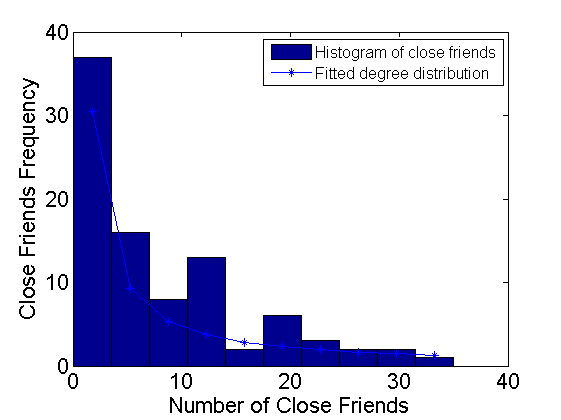
\includegraphics[scale = 0.9]{friends_distribution_figure1.png}
   \caption{\label{1} Average degree distribution of close friends}
\end{figure}

\paragraph{}
The parameters of the power law fitted function y=\alpha x^\beta \]   are \alpha=55 \] and \beta=-1.07\].

\paragraph{}
We then test two types of assortativity: social assortativity and weight assortativity. We run the regression of the average nearest neighbor degree against the average degree of a subject to test the social assortativity of the network. The Friends and Family network is socially assortative as shown in Figure 3as subjects with a higher number of close friends tend to have a higher nearest neighbor degree.We find a positive coefficient on the average degree equal to 0.34 and significant at the 5\% level.


\begin{figure}[!h]
\center
   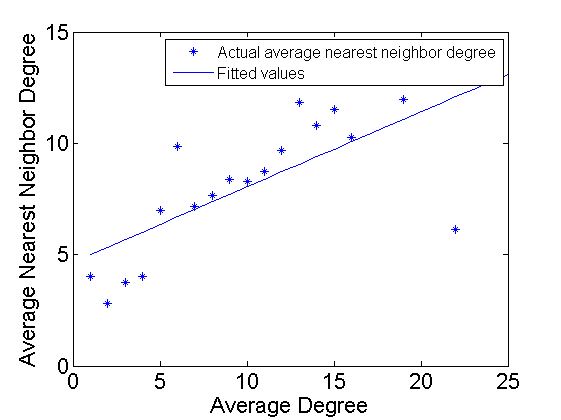
\includegraphics[scale=0.72]{social_assortativity_figure2.png}
   \caption{\label{2} Friends and Family Network Social Assortativity.}
\end{figure}

\paragraph{}
However we do not obtain significant results to support weight assortativity when running the regression of the average nearest neighbor weight against a subject's weight (see Figure 3). The coefficient of the regression slope of the average nearest neighbor weight against a subject weight is not significant at any conventional level. We therefore conclude that a subject weight is not associated with its average nearest neighbor weight. 

\begin{figure}[!h]
\center
   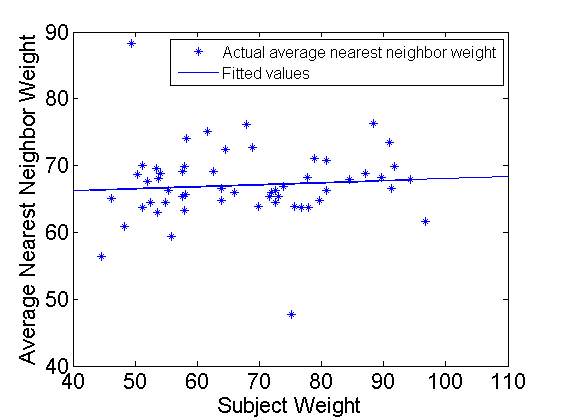
\includegraphics[scale=0.72]{weight_assortativity_figure3.png}
   \caption{\label{3} Friends and Family Network Weight Assortativity.}
\end{figure}


\subsection{Regression results}
\paragraph{}
Our findings relate in parts to the outcome of the analysis of Christakis. We solved to some extent the question raised in his talk at Dartmouth College in 2008 concerning the outcome in a different socio-economic environment, where perception of obesity is different. But when we used the body fat metric which is reportedly a more precise measure for obesity, we surprisingly did not encounter neater proof of the infectious characteristic of obesity, as we find a negative correlation. What's more, we determined in multiple tests that running the regression with even a small shift in the threshold value triggering a change of state, yielded a great impact in the outcome, even negating the correlation when ran against the body fat measure. This surprising mismatch between BMI and body fat, which normally relate to each other in terms of the following approximation formula for an adult: 
\[Adult Body Fat \% = (1.20 * BMI) + (0.23 * Age) - (10.8 * gender) - 5.4\]
, is, as far as we can tell, due to the remarkably high skeletal muscle percentage of the total weight reported by the study participants. This reflects the fact that the study participants were drawn from a university setting, where university athletes are overrepresented compared to the general population. 

\paragraph{}
To determine the parameters of the differential systems, we have made a regression over the percentage of change from one state to another given the number of contacts in the target state. The obtained p-values are high. The smaller p-value we get is indeed 0.306 for the study of the BMI with a threshold put at 25. The parameters we get this way do not seem reliable. 

\paragraph{}

Overall, we could not prove the thesis that obesity and overweight spread like a contagious disease nor refute it, and prove that the healthy state spreads, as in both ways the correlation was too small, especially given our small study sample of 85 subjects and the short time scale of 145 days, i.e. less than five months.

\subsection{Simulation results}
\paragraph{}
The simulation parameters resulting of the regression on our data yielded a long term prevalence of obesity when inspecting BMI. When we looked at the body fat percentage, the outcome was different, with the healthy state of normal weight becoming dominant.

%[Add the graph of the evolution of the number of the persons above threshold plot(sum(PersonID_x_AboveAtExam))

\paragraph{}
The evolution of the number of persons above a given threshold of BMI is strongly dependant on the threshold given but tend to grow. In order to observe if the SISa model could fit this data with any parameter, we calculated %% TO BE FINISHED


\subsection{Importance of the a parameter in a SISa model}
\paragraph{}
To tell things upfront, the SISa model is very sensible to the value of each single value, with the ration of \beta  \] /g being the most prevalent. As we can infer from the following graphs, a single decimal change can yield noticeable different outcomes.



\subsection{Society implication}
\paragraph{}
The society implication of clearly understanding the to what extent and in which manner social spreading of obesity happens are huge. Given that it is morally unacceptable to marginalize obese people and even the small direct correlation is hard to link causation, we prone a more holistic approach were obesity is seen as a risk factor as opposed to a disease . Thus this risk factor has to be contained through environmental reforms on one hand like easier access to sport facilities, bike to work initiatives, promotion of healthier food alternatives in canteen settings, and social reforms on the other hand where risk reduction due to obesity is rewarded and scheduled physical activity is integrated in the daily work routine. Politics also have to play a role as they did with the tobacco advertisement restrictions and warning by translating these efforts to the junk food advertisement restrictions and clearer formulated food declaration, lobbying for "junk food free" as they did for smoke free.

\subsection{Limitations}
\paragraph{}
Despite Aharony et al. claims, the Friends and Family network does not appear to be representative of the US population as all subjects were members of a residential living community living next to MIT. The BMI distribution of the Friends and Family netwoek does not reflect the BMI distribution of the entire US population. Flegal et al. have found a prevalence of obesity of 35\% among US adults. In comparison, the mean BMI in the Friends and Family network is 23 and 5 out of the 85 subjects are obese in the sample at the beginning of the study.

\begin{figure}[!h]
\center
   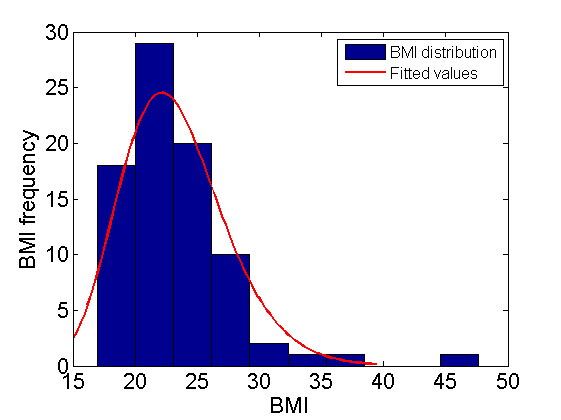
\includegraphics[scale = 0.9]{bmi_distribution_figure4.png}
   \caption{\label{4} BMI distribution of the Friends and Family network. A lognormal distribution is fitted to the BMI data with a mean of 3.13 and standard deviation of 0.18.}
\end{figure}


\paragraph{}

Another factor that a model purely based on social contagion does not capture is the alimentary culture that is not directly related to social interaction but largely shared across a social group. Some populations, and therefore the social networks they span, are much more at risk of a deregulation of equilibrium in their macronutrient intake, struggling to cover their protein needs while increasing their overall calories consumption. 

\paragraph{}
We take into account Shalizi and Thomas comments regarding environmental confounding and decided to examine the role of socio-environment in obesity. Using data from the US Department of Agriculture, we run a regression of the 2010 obesity prevalence in 3'137 US counties against the median household income in USD'000 of these same counties. These results highlight the role of confounding and support the argument of Shalizi and Thomas as we find a negative coefficient on the median household income in USD'000 equal to -0.19 and statistically significant at all conventional level. One possible explanation for this is that low income families might consume lower quality food which often contains more fat because of budget constraints.

\section{Summary and Outlook}

\section{References}
\paragraph{}
Aharony, N., Pan, W., Ip, C., Khayal, I., \& Pentland, A. (2011). Social fMRI: Investigating and shaping social mechanisms in the real world. Pervasive and Mobile Computing, 7(6), 643–659.
\paragraph{}
Barabási, A.-L. (2009). Scale-free networks: a decade and beyond. Science, 325(5939), 412–413.
\paragraph{}
Christakis, N. A., \& Fowler, J. H. (2007). The spread of obesity in a large social network over 32 years. New England Journal of Medicine, 357(4), 370–379.
\paragraph{}
Flegal, K. M., Carroll, M. D., Kit, B. K., \& Ogden, C. L. (2012). Prevalence of obesity and trends in the distribution of body mass index among US adults, 1999-2010. Jama, 307(5), 491–497.
\paragraph{}
Flegal, K. M., Williamson, D. F., Pamuk, E. R., \& Rosenberg, H. M. (2004). Estimating deaths attributable to obesity in the United States. American Journal of Public Health, 94(9), 1486.
\paragraph{}
Hill, A. L., Rand, D. G., Nowak, M. A., \& Christakis, N. A. (2010). Infectious disease modeling of social contagion in networks. PLoS Computational Biology, 6(11), e1000968.
\paragraph{}
Kermack, W. O., & McKendrick, A. G. (1932). Contributions to the mathematical theory of epidemics. II. The problem of endemicity. Proceedings of the Royal Society of London. Series A, 138(834), 55–83.
\paragraph{}
Shalizi, C. R., & Thomas, A. C. (2011). Homophily and contagion are generically confounded in observational social network studies. Sociological Methods & Research, 40(2), 211–239.
\paragraph{}
Smith, K. P., & Christakis, N. A. (2008). Social networks and health. Annu. Rev. Sociol, 34, 405–429.

\section{Annexes}
\subsection{Code listing}
\paragraph{File Project\_script.m}
\begin{verbatim}
    load('DATA.mat')
    prompt = 'What variable do you want to study? Type BMI or body_fat  ';
    studied_variable = input(prompt);
    prompt = 'Choose a meaningful threshold for the variable:';
    threshold = input(prompt);
    % Generate adjancency matrix of subjects
    [adj_mat,adj_mat_bin,unique_source,unique_target] = mssmm_adj(participantID_weight,participantID_weight,source_friendship,date_friendship_can);
    % Degree distibution in the network
    [contacts,avg_degree] = degree_distribution(adj_mat_bin);
    disp(avg_degree);
    % Is the ego above the threshold at the exam:
    PersonID_x_AboveAtExam = persons_above_interpolated( participantID_weight,studied_variable, date_weigth_can,threshold);
	%Plots the evolution of the number of person above
    figure(1)
    plot(sum(PersonID_x_AboveAtExam)/size(PersonID_x_AboveAtExam,1))
	% When did a transition from one state to the next happen and which way:
    PersonID_x_ChangedStateAtDayX = persons_changed_state( PersonID_x_AboveAtExam );
    % Number of contacts above the threshold at the exam:
    [number_of_contacts] = count_obese_contacts(PersonID_x_AboveAtExam, adj_mat_bin);
    % Percentage of total transitions happening given a count of contacts
    % above the threshold:
    change_under = mssmm_regression(PersonID_x_ChangedStateAtDayX, number_of_contacts, sum(adj_mat_bin(:,:,1)),true)
    change_above = mssmm_regression(PersonID_x_ChangedStateAtDayX, number_of_contacts, sum(adj_mat_bin(:,:,1)),false)
    % regression on the parameters
    [above b g a] = mssmm_regression_results(change_above, change_under)
    % plot regression results
    figure(2);
    plot(change_above(:,1),change_above(:,2))
    hold on;
    x = change_above(:,1);
    y = b*x+a;
    plot(x,y*100,'o');
    hold off;
    initial_infected = sum(PersonID_x_AboveAtExam(:,1)) * (100 / size(PersonID_x_AboveAtExam,1));
    figure(3);
    [susceptible,infected] = simulation(a,b,g, initial_infected, size(PersonID_x_AboveAtExam,2), 0.01);

% Discussed tests: studied_variable=BMI, threshold=26: slight correlation,
% ~stable state at 75% infected
% Second test: studied_variable=body_fat, threshold=25: apparent negative correlation,
% ~stable state at 15% infected
% Third test: studied_variable=BMI, threshold=25: some correlation,
% ~stable state at 90% infected
% Fourth test: studied_variable=body_fat, threshold=25: apparent negative correlation,
% ~stable state at 12% infected

\end{verbatim}
\paragraph{File mssmm\_adj.m}
\begin{verbatim}
function [adj_mat,adj_mat_bin,unique_source,unique_target,unique_funf_group]=mssmm_adj(source,target,source_friendship,date_friendship_can)
    %% Returns the adjacency matrix, a binary adjacency matrix, a vector of unique elements of source and target
    % Input: 
        % source is the vector source in FunFit Excel file, target is
        % the vector source in FunFit Excel file, source_friendship is the
        % vector source_friendship in SurveyFriendship Excel file, date_friendship is the
        % vector date_friendship in SurveyFriendship Excel file
        % self-reported friendship ranging from 0 to 7. The binary
        % adjacency matrix displays 1 when the the self reported
        % friendship > 2
    % Output:
        % adj_mat is a  3D adjacency matrix matrix, the first two dimensions corresponds to
        % the person and the third dimension to the date of friendship
        % unique_source is the vector of unique source (idem for
        % unique_target)
    
    load('DATA.mat')
    %% Vector of unique source
        unique_source= unique(participantID_weight);%zeros(1,1);
        number_of_egos = length(unique_source) % for logging
    %% Vector of unique target
        unique_target= unique(participantID_weight);%zeros(1,1);
        %length(unique_target)
        
    %% Return the experiment to which a person belongs (Control,See-Peer,Pay-Peer)
    % unique_funf_group=cell(length(unique_source),1);
    % for i=1:length(unique_source)    
    %     funf_group_index=find(ismember(source,unique_source(i)));
    %     unique_funf_group{i}=funf_group{funf_group_index};
    % end
       
    %% Creation of the adjacency matrix
 
    date=unique(date_friendship_can);
    adj_mat=zeros(length(unique_source),length(unique_target),length(date));
    adj_mat_bin=zeros(length(unique_source),length(unique_target),length(date));

    for i=1:length(source_friendship)

        % source_friendship_index returns index of person in the adjacency matrix
        source_friendship_index=find(ismember(unique_source,source_friendship(i)));
        target_friendship_index=find(ismember(unique_target,target_friendship(i)));
        date_index=find(ismember(date,date_friendship_can(i)));

        % Adjacency matrix element value equal to weight_friendship
        % value ranges from 0 to 7
        adj_mat(source_friendship_index,target_friendship_index,date_index)=weight_friendship(i);
        if weight_friendship(i)>2
            adj_mat_bin(source_friendship_index,target_friendship_index,date_index)=1;% binary adjacency matrix 1
        else
        end

    end
end

\end{verbatim}

\paragraph{File degree\_distribution.m}
\begin{verbatim}
function [contacts,avg_degree]=degree_distribution(adj_mat_bin)
    %% Returns the degree distribution (distribution of contact numbers) of the network at each time
    
    % Input:
            % Binary adjacency matrix: 1 if person are close friends and 0
            % otherwise
    % Ouput:
            % number_of_contacts matrix with the number of contacts of each person at the
            % each time
            % The plots displays the degree distribution histogram
            
    date=size(adj_mat_bin,3); % number of date
    len_source=size(adj_mat_bin,1); % number of persons
    
    contacts=zeros(len_source,date);
    avg_degree=zeros(date,1);
    
    for t=1:date
        for k=1:len_source
            contacts(k,t)=sum(adj_mat_bin(k,:,t)); % Number of close friends of person k at time t 
        end

        total_contacts=sum(contacts(:,t));
          
        % figure

        % bar(1:max(number_of_contacts(:,t)),1/total_contacts*histc(number_of_contacts(:,t),1:max(number_of_contacts(:,t))),'histc')% Histogram of degree distribution
        
        % figure
        
        avg_degree(t,1)=total_contacts/len_source;
        % hist(number_of_contacts(:,t))% Histogram of degree distribution
        % xlabel('Number of close friends')
        % ylabel('Close friends frequency')
        % title(['Close friends distribution t=',num2str(t)],'FontSize',10,'fontweight','bold')
        
    end
 
end
\end{verbatim}

\paragraph{File persons\_above\_interpolated.m}
\begin{verbatim}
function PersonID_x_AboveAtExam = persons_above_interpolated( persons, vector_measure, date_measure, threshold)
    % SUMMARY: persons_above computes for each unique person if they are above the
    %threshold at a given day.
    %
    % OUTPUT:: PersonID_x_AboveAtExam : Returns a unique_persons by
            % first_date_of_measure_to_last_date_of_measure matrix with value 1 if above
            % the threshold and 0 else.
    % INPUT::
        % persons: a vector of cells of personID strings,
        % vector_measure: a vector of numeric values, where value at row x
        % corresponds to person at row x.
        % date_measure: a vector of dates in integer form, where value at row x
        % corresponds to measure at row x.
        % threshold: a threshold above which the state is 1.

    egos = unique(persons); % different persons
    duration = max(date_measure)-min(date_measure) + 1; % Time elapsed from first measurement (inclusive) to last measurement (inclusive)
    date_measure = date_measure - min(date_measure) + 1; % normalize date_weight

    PersonID_x_AboveAtExam = zeros(length(egos),duration); % make empty

    %warning('off', 'MATLAB:polyfit:RepeatedPointsOrRescale'); % temporarly turn off those warnings about badly conditioned polynomials

    for i= 1:length(egos)
        personInd = find(ismember(persons,egos(i))); % personInd = person indexes

        measureDateEgo = date_measure(personInd); % We need the indexes corresponding to a person sorted by date, in order to compute the final matrix in one pass per person.
        dates_measures = [measureDateEgo, personInd]; % Prepend date vector to index vector
        dates_measures = sortrows(dates_measures); % Sort after date vector
        mbd = dates_measures(:,2); % extract sorted by date index vector of the measures i.e. MeasuresByDate
        measureDateEgo = dates_measures(:,1); % dates sorted

        person_measures = vector_measure(mbd); % all the measures of an ego
        % remove multiple measurements that were taken on the same day to
        % avoid badly conditioned polynomial
        [measureDateEgo, index_measureDateEgo, ~] = unique(measureDateEgo,'stable');
        person_measures = person_measures(index_measureDateEgo);
        measure_count = length(measureDateEgo);
        degree = min(measure_count-1, 1); % restrict polynom to degree <= 2 to avoid edge effects
        p = polyfit(measureDateEgo,person_measures,degree);
        x = 1:duration;
        y = polyval(p,x);
        plot(x,y);


        y(y <= threshold) = 0; % binary matrix: 0 -> value below threshold at this date for this person
        y(y > threshold) = 1; % binary matrix: 1 -> value above or equal threshold at this date for this person
        PersonID_x_AboveAtExam(i,:) = y;
    end
end

\end{verbatim}

\paragraph{File persons\_changed\_state.m}
\begin{verbatim}
function PersonID_x_ChangedStateAtDayX = persons_changed_state( PersonID_x_AboveAtExam )
%SUMMARY: persons_changed_state computes for each unique person if they changed
%state with respect to previous day.
%
% OUTPUT:: PersonID_x_ChangedStateAtDayX : Returns a unique_persons by
        % first_date_of_mesure_to_last_date_of_mesure matrix with value 0 if the person doesn't changed state with respect to previous day.
        % If the person state changed from under the threshold to above the
        % threshold on the next day, the value is -1.
        % If the person state changed from above the threshold to under the
        % threshold on the next day, the value is 1.
% INPUT::
        % PersonID_x_AboveAtExam

[m,n] = size(PersonID_x_AboveAtExam);

PersonID_x_ChangedStateAtDayX = [zeros(m,1),PersonID_x_AboveAtExam(:,1:n-1)] - [zeros(m,1),PersonID_x_AboveAtExam(:,2:n)];

end

\end{verbatim}

\paragraph{File count\_obese\_contacts.m}
\begin{verbatim}
% function returns a matrix 'number_of_obese_contacts'
% that has the number of obese contacts each person has at every timestep
% weight_over_time: entry (i,j) represents whether person i is obese at
% time j (entry in the matrix is one) or not (entry is zero)
% adj matrix, entry (i,j) represents whether person i knows person j or not
function [number_of_obese_contacts] = count_obese_contacts(weight_over_time, adj_matrix)
    number_of_persons = size(weight_over_time,1);
    time_steps = size(weight_over_time,2);
    number_of_obese_contacts = zeros(number_of_persons, time_steps);
    for i = 1:number_of_persons
        for j = 1:number_of_persons    
            if adj_matrix(i,j)>=1     %check if person i is in relation with person j
                for k = 1:time_steps   % at any time step if person 'j' is obese, increment the number of obese contacts of person 'i' by one at that time step
                    if weight_over_time(j,k)>=1
                        number_of_obese_contacts(i,k) = number_of_obese_contacts(i,k) +1; 
                    end
                end
            end
        end
    end
end

\end{verbatim}

\paragraph{File mssmm\_regression.m}
\begin{verbatim}
function changes =mssmm_regression(persons_changed_states, count_contacts_above, number_contacts, under_to_above)
 % SUMMARY: Compute the number of changes from under to above (or under) the threshold value
 % with respect to the number of contacts under (or above) threshold at the time step
 % of the change
 
 %OUTPUT :: A matrix of two columns. The first one corresponds to the number of contacts observed
 % the second one to the percentage of the changes that took place in this particular configuration of contacts
 
 %INPUT ::
 % persons_changed_state : output of the function persons_changed_state
 % (Returns a unique_persons by
 % first_date_of_mesure_to_last_date_of_mesure matrix with absolute value 1
 % if the person changed state with respect to previous day and 0 else.)
 % count_matrix_above : output of the count_matrix function
 % number_contacts : column vector with the total number of contacts of
 % each person
 % under_to_above : boolean value. if TRUE, then changes from under_to_above ; else
 % then compute the changes from state above to state under threshold

 
 pcs = -persons_changed_states;
 contacts_new_state = count_contacts_above;
 
 if ~(under_to_above)
     pcs = persons_changed_states;
     number_contacts = transpose(number_contacts);
     n = size(count_contacts_above, 2);
     contacts_new_state = repmat(number_contacts, 1, n)-contacts_new_state;
 end
 
 changes_with_counts = tabulate(uint8(contacts_new_state(pcs>0)));
 changes = changes_with_counts(:,[1 2]);
 changes(:,2) = changes(:,2)/size(persons_changed_states,1);
   
end

\end{verbatim}

\paragraph{File mssmm\_regression\_results.m}
\begin{verbatim}
function [above b g a] =mssmm_regression_results(change_above, change_under)
 % SUMMARY: Compute the parameters to be used in the SIS and SISa model
 
 %OUTPUT :: The parameters to be used in the SIS model and SISa model, by
 %determining the state that is infectious ( cf. Hill and al.)
 % above : boolean variable. 1 if above is the infectious state. 0 if under
 % is the infectious state
 
 %INPUT ::
 % changes_above : output of the function msssm_regression on the changes
 % from the under threshold state to the above threshold state
 % changes_under : output of the function msssm_regression on the changes
 % from the above threshold state to the under threshold state
 
 
 x_above = change_above(:,1);
 y_above = change_above(:,2)/100;
 
 x_under = change_under(:,1);
 y_under = change_under(:,2)/100;
 
 lin_above = fitlm(x_above, y_above, 'linear') % use GeneralizedLinearModel.fit instead of firlm in versions prior to MatLab R2014a
 lin_under = fitlm(x_under, y_under, 'linear')
    
 coef_above = cell2mat(table2cell(lin_above.Coefficients));
 coef_under = cell2mat(table2cell(lin_under.Coefficients));
 
 if double(coef_under(2,4)) > double(coef_above(2,4)) % Corresponds to a comparison of the p-value
     above = 1;
     b = double(coef_above(2,1));
     a = double(coef_above(1,1));
     g = change_under(1,2);
 else
     above = 0;
     b = double(coef_under(2,1));
     a = double(coef_under(1,1));
     g = change_above(1,2);
 end

end

\end{verbatim}

\paragraph{File simulation.m}
\begin{verbatim}
function [susceptible,infected] = simulation(a,b,g, initial_infect, duration, step)
    % SUMMARY: Simulates the SISa model for the automatic (or spontaneous)
    % infection factor a, the transmission rate b, and the recovery rate g,
    % for an initialy infected percentage of initial_infect, a duration of
    % 'duration' days, with a resolution in the timesteps of step.
    
    % OUTPUT::
            %susceptible vector with the susceptible percentage per timestep
            % infecter vector with the infected percentage per timestep
    % INPUT::
            %parameters: a=spontaneous infection rate; b=transmission rate; g=recovery
            %rate; duration=duration of the simulation; step=time step
            
    dt=step;        % time step, initialise manually here when desired
    d = duration;   % simulated duration, initialise manually here when desired

    % initial condition
    S=100-initial_infect;      % Susceptible egos
    I=initial_infect;   % Infected individualsS
    % book-keeping variable
    index = 0;

    % simulation loop
    for t=1:dt:d+1
        index = index + 1;
        dI = (b*S*I-g*I+a*S)*dt;
        dS = (-b*S*I+g*I-a*S)*dt;
        I = I + dI;
        i(index) = I;
        S = S + dS;
        s(index) = S;
    end
    format short
    x = linspace(1,t,(d/dt)+1);
    plot(x,s)
    grid on
    hold on
    plot(x,i,'o')
    hold off
    infected = i;
    susceptible = s;
end

\end{verbatim}

\end{document}  
